\subsection{Case04 - Layer 3 forwarding}
\label{P4_ether_case04}

En este caso de uso, se abordará la implementación un forwarding a nivel de red, capa 3, por lo que el hipotético ``switch" será ahora un un router muy básico y con muy pocas funcionalidades. Por ello conviene recordar las anotaciones que se hicieron sobre el \gls{bmv2} y por qué no debemos definirlo únicamente como un soft-switch, ya que depende del programa P4 que porte para definir su \textit{datapath} y su interfaz con el plano de control.\\
\par

La motivación de este caso de uso, es ver el equivalente en P4 que tiene el código de retorno \gls{xdp} llamado \texttt{XDP\_REDIRECT}. En el anterior caso de uso ya se hacía uso de la información de metadatos para elegir el puerto de salida del paquete. Por lo que podríamos afirmar que este es el equivalente directo al forwarding en \gls{xdp}, solo que aquí en P4 resulta más sencillo ya que únicamente indicamos por número de puerto mientras que \gls{xdp} se debía obtener el \textit{ifindex} de la interfaz a la cual íbamos a hacer el reenvío. Como se puede apreciar en la figura \ref{code:case04_p4_ether_prog1}, unicamente le indicamos el puerto por el cual debe salir el paquete.\\
\par

\begin{lstlisting}[language=C, style=P4-color, caption={Redirección del paquete - Case04},label=code:case04_p4_ether_prog1]
    standard_metadata.egress_spec = port
\end{lstlisting}
\vspace{0.5cm}

Pero, ¿Qué son los números de puerto? ¿Cuando se han establecido estos identificadores? Estos números de puerto se establecen cuando se levanta la instancia del \gls{bmv2}. Se asocia interfaz real con un número identificativo. Serán estos números identificativos los números de puerto de cada ``switch". De esta manera el ``switch" tiene a su alcance todos sus posibles puertos. El levantamiento de las instancias de \gls{bmv2} se llevan a cabo con la carga del script \texttt{run\_exercise.py}. Este a su vez hace uso de la clase \texttt{P4RuntimeSwitch} definida en la interfaz de Python hacia Mininet,  para levantar dicho ``switch" pasándole los parámetros adecuados. Se puede levantar una instancia del \gls{bmv2} siguiendo las indicaciones del bloque \ref{code:case04_p4_ether_instacia}.\\
\par

\begin{lstlisting}[language= bash, style=Consola, caption={Ejecución de instancia del BMv2 - Case04},label=code:case04_p4_ether_instacia]
    sudo simple_switch_grpc --log-console --dump-packet-data 64 \
                        –i 0@veth0 -i 1@veth2 … [--pcap] --no-p4 \
                        --grpc-server-addr 0.0.0.0:50051 --cpu-port 255 \
                        test.json
\end{lstlisting}
\vspace{0.5cm}
Una vez entendido de dónde salen los números de puerto, se debe plantear la siguiente cuestión, ¿Cómo un programa P4 es capaz de conocer los posibles puertos de los que puede disponer para reenviar un paquete?\\
\par
No puede, y tampoco es lógico que en un programa P4, donde se define el \textit{datapath}, ya estén preestablecidos los números de puerto posibles a manejar. Ya que si eso fuera así, se tendría que tener distintos programas P4 por cada entidad con un número de puertos distintos (únicamente para implementar un único \textit{datapath}). No es viable. Por ello, toda la información relativa a los puertos, asociada al forwarding, generalmente suele venir desde el plano de control quien tiene constancia de los puertos de dicho ``switch".\\
\par

Por ejemplo, si se quiere hacer forwarding de un paquete a un puerto en especifico dado su IP, necesitaremos que el plano de control indique el criterio a seguir, qué IPs están asociadas a según que puertos. Esta interfaz entre el plano de datos y el plano de control esta definidas por tablas.\\
\par

Desde el programa P4 se tiene que definir el esqueleto de la tabla, indicando qué \textit{actions}
están disponibles, qué parámetros reciben esas \textit{actions}, qué criterio de match tendrá la tabla, sobre qué \textit{keys} se realizará el \textit{lookup} y cuál es el número máximo de entradas en dicha tabla. A continuación, se muestra la figura \ref{fig:case03_p4_ether_tablas} que resume bastante bien la funcionalidad de las tablas.\\
\par

% figura escenario
\begin{figure}[ht]
    \centering
    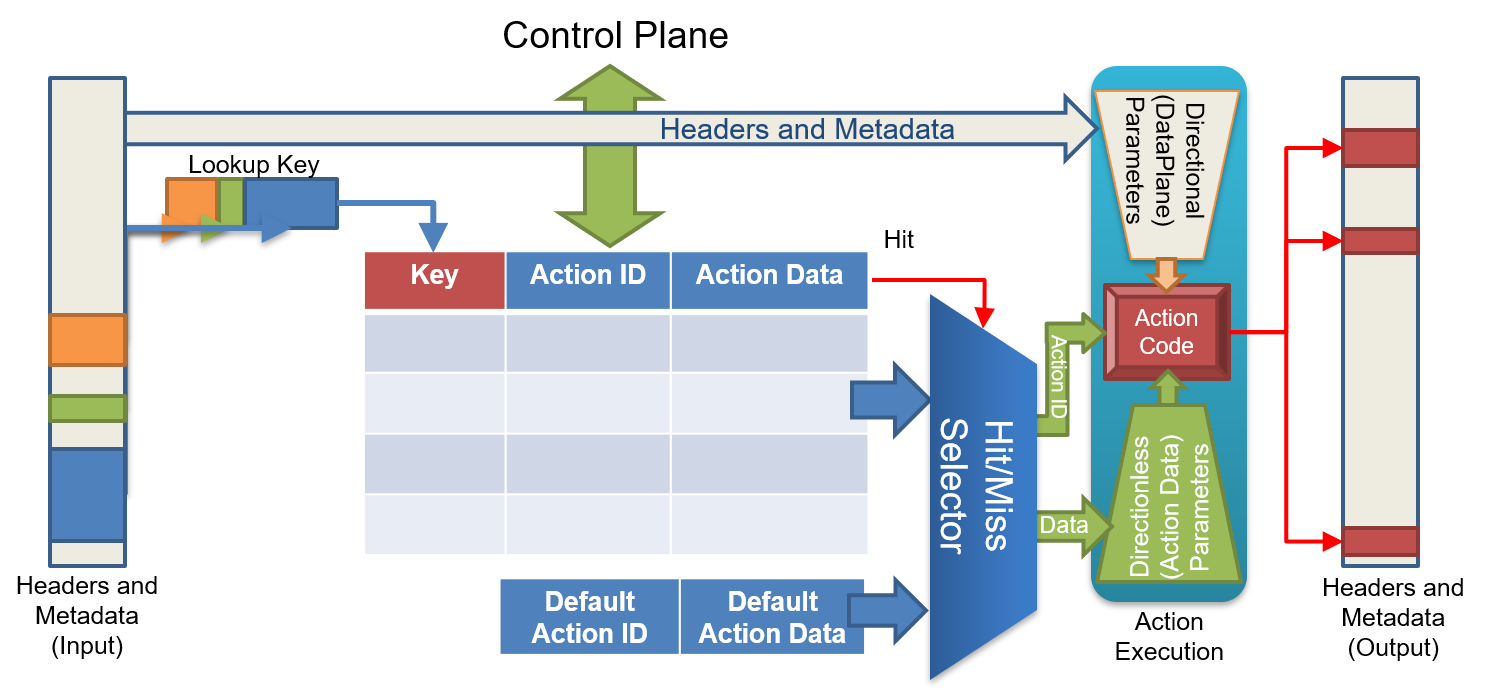
\includegraphics[width=16cm]{archivos/img/dev/p4/case04/table.png}
    \caption{Funcionamiento de las tablas en P4 \cite{p42}}
    \label{fig:case03_p4_ether_tablas}
\end{figure}
\vspace{0.2cm}

Por tanto, desde el plano de control, bien vía P4Runtime ó vía json con los ficheros \texttt{sX-runtime.json} (que se cargarán a través de la CLI-\gls{bmv2}), se rellenarán las entradas de dicha tabla y los parámetros de las acciones a llevar a cabo cuando haya un \textit{hit} con dicha entrada. En este caso se asociarán IPs a una acción de forwarding donde  se le  suministrará por qué puerto tiene que salir el paquete y que MAC destino debe llevar.\\
\par

Una vez entendidos los números de puerto y el concepto de las tablas, se debe abordar el cómo hacer una acción de forwarding para reenviar los paquetes que lleguen al \gls{bmv2}. Esta acción de forwarding deberá se capaz de actualizar el puerto de salida, actualizar la MAC destino y decrementar en uno el campo \texttt{ttl} de la cabecera IP. A continuación, se indica la acción propuesta para llevar a cabo dicho cometido (Ver bloque \ref{code:case04_p4_ether_prog1}).

\begin{lstlisting}[language=C, style=P4-color, caption={Acción propuesta para llevar a cabo el forwarding - Case04},label=code:case04_p4_ether_prog2]
    /*
     * Se quiso hacer uso del operador '-=' pero la sintaxis de P4 no lo permite :(
     */
    
    action ipv4_forward(macAddr_t dstAddr, egressSpec_t port) {
            standard_metadata.egress_spec = port;
            hdr.ethernet.srcAddr = hdr.ethernet.dstAddr;
            hdr.ethernet.dstAddr = dstAddr;
            hdr.ipv4.ttl = hdr.ipv4.ttl - 1;
    }
\end{lstlisting}
\vspace{0.5cm}
Teniendo la acción ya disponible, solo quedaría aplicar la tabla en nuestra pipeline del programa P4 y ya se estaría haciendo un forwarding en capa 3.

\vspace{0.5cm}
\textbf{Compilación y puesta en marcha del escenario}\\
\par

Para la compilación del programa P4 se hará uso del compilador P4c (más información sobre el proceso de compilación en la subsección \ref{p4_ether_case01}).\\
\par

Dado que las personas que quieran replicar los casos de uso puede que no estén muy familiarizadas con todo este proceso de compilación y carga en los procesos de \gls{bmv2}, se ha dispuesto un de un Makefile para automatizar las tareas de compilación y carga, y las tareas de limpieza del caso de uso. Entonces para la puesta en marcha del caso de uso se deben seguir los pasos indicados en el bloque \ref{code:case04_p4_ether_load}.

\begin{lstlisting}[language= bash, style=Consola, caption={Compilación programa P4 y puesta en marcha del escenario - Case04},label=code:case04_p4_ether_load]
    # Entramos al directorio 
    cd TFG/src/use_cases/p4/case04

    # Hacemos uso del Makefile
    sudo make run
\end{lstlisting}
\vspace{0.5cm}

Una vez se haya finalizado la comprobación del funcionamiento del caso de uso, se debe hacer uso de otro target (\textit{clean}) del Makefile para limpieza total del directorio según se indica en el bloque \ref{code:case04_p4_ether_unload}.

\begin{lstlisting}[language= bash, style=Consola, caption={Limpieza del escenario P4 - Case04},label=code:case04_p4_ether_unload]
    # Hacemos uso del Makefile
    sudo make clean
\end{lstlisting}
\vspace{0.5cm}

Es importante señalar que este target limpiará tanto los ficheros auxiliares para la carga del programa P4 en el \gls{bmv2}, como los directorios de \texttt{pcaps}, \texttt{log}, y \texttt{build} generados en la puesta en marcha del escenario. Por lo que si se desea conservar las capturas de las distintas interfaces de los distintos \gls{bmv2}, cópielas o haga la limpieza del escenario a mano siguiendo las indicaciones del bloque \ref{code:case04_p4_ether_unload2}.
\begin{lstlisting}[language= bash, style=Consola, caption={Limpieza segura del escenario P4 - Case04},label=code:case04_p4_ether_unload2]
    # Limpiamos Mininet
    sudo mn -c
    
    # Limpiamos los directorios generados dinámicamente en la carga del escenario
    sudo rm -rf build logs
\end{lstlisting}


\vspace{0.5cm}
\textbf{Comprobación del funcionamiento}\\
\par


Así pues, después de realizar el \texttt{make run} en este directorio, se tendrá levantada la topología descrita para este caso de uso, la cual se puede apreciar en la figura \ref{fig:case04_p4_ether_scenario}. Como en el \textit{datapath} no se contempla el manejo de ARP, se ha añadido el ARP entry a directamente desde el fichero \texttt{topology.json} consiguiendo así que no se genere la resolución ARP en el envío de los \texttt{ECHO-Request}. Este arreglo es poco elegante ya que se le está indicando un hipotético \textit{gateway} que no existe, y se está añadiendo un ARP entry con la MAC de dicho \textit{gateway}. De esta forma, todos los paquetes saldrán con la MAC destino indicada en la entry y no se producirá la resolución ARP. Al llegar al ``switch" el paquete verá modificada su MAC destino en función de su IP destino, por lo que la ``chapuza" no irá a más.\\
\par

% figura escenario
\begin{figure}[ht]
    \centering
    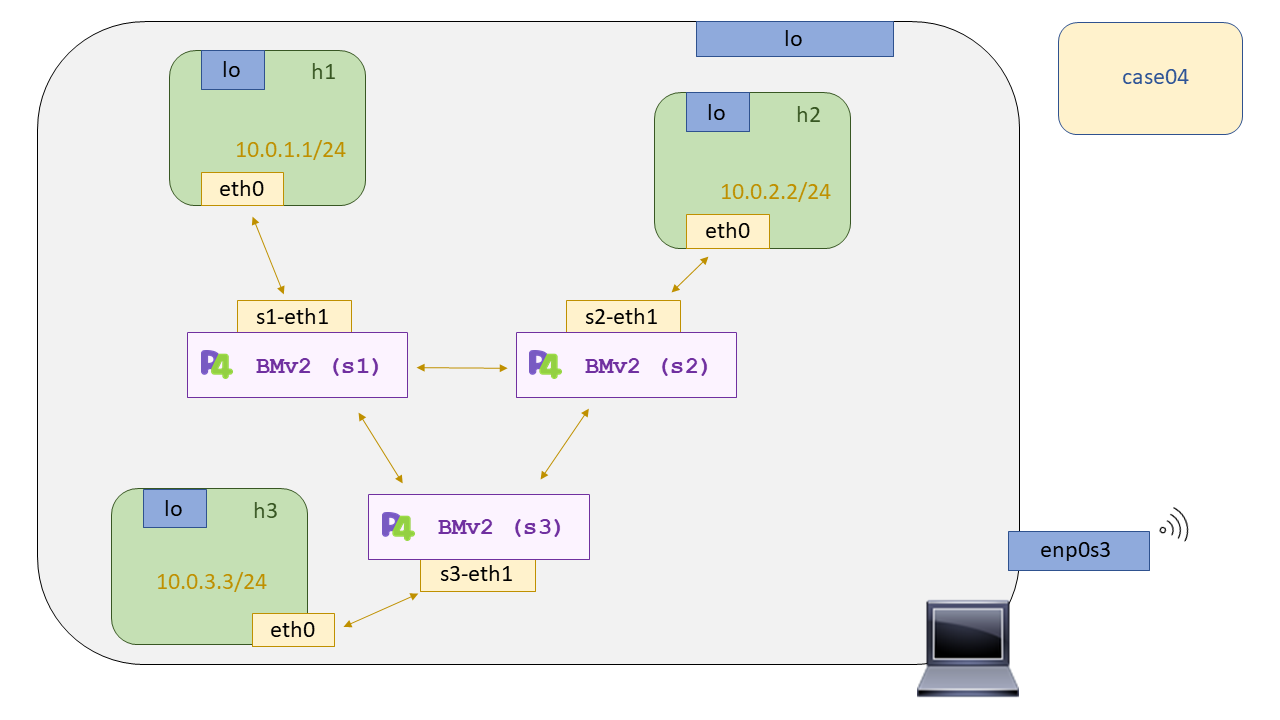
\includegraphics[width=12cm]{archivos/img/dev/p4/case04/scenario.png}
    \caption{Escenario del Case04 - P4}
    \label{fig:case04_p4_ether_scenario}
\end{figure}


Volviendo de nuevo a la comprobación del funcionamiento del caso de uso, se tendrá la CLI de Mininet abierta, por lo que simplemente se probará la conectividad entre todos los hosts. Esto se puede realizar ejecutando la orden \texttt{pingall}, la cual ejecutará pings entre todos los hosts, comprobando así la conectividad bidireccional de todos los \textit{paths} preestablecidos en el escenario. De forma adicional, se podría hacer uso de un \textit{sniffer} para comprobar que los paquetes llegan con el campo \texttt{ttl} modificado, en función de los saltos que ha dado el paquete. Según se puede apreciar en la figura \ref{fig:case04_p4_ether_func}, hay perfecta conectividad entre todos los hosts de la topología.

\newpage

% figura escenario
\begin{figure}[ht]
    \centering
    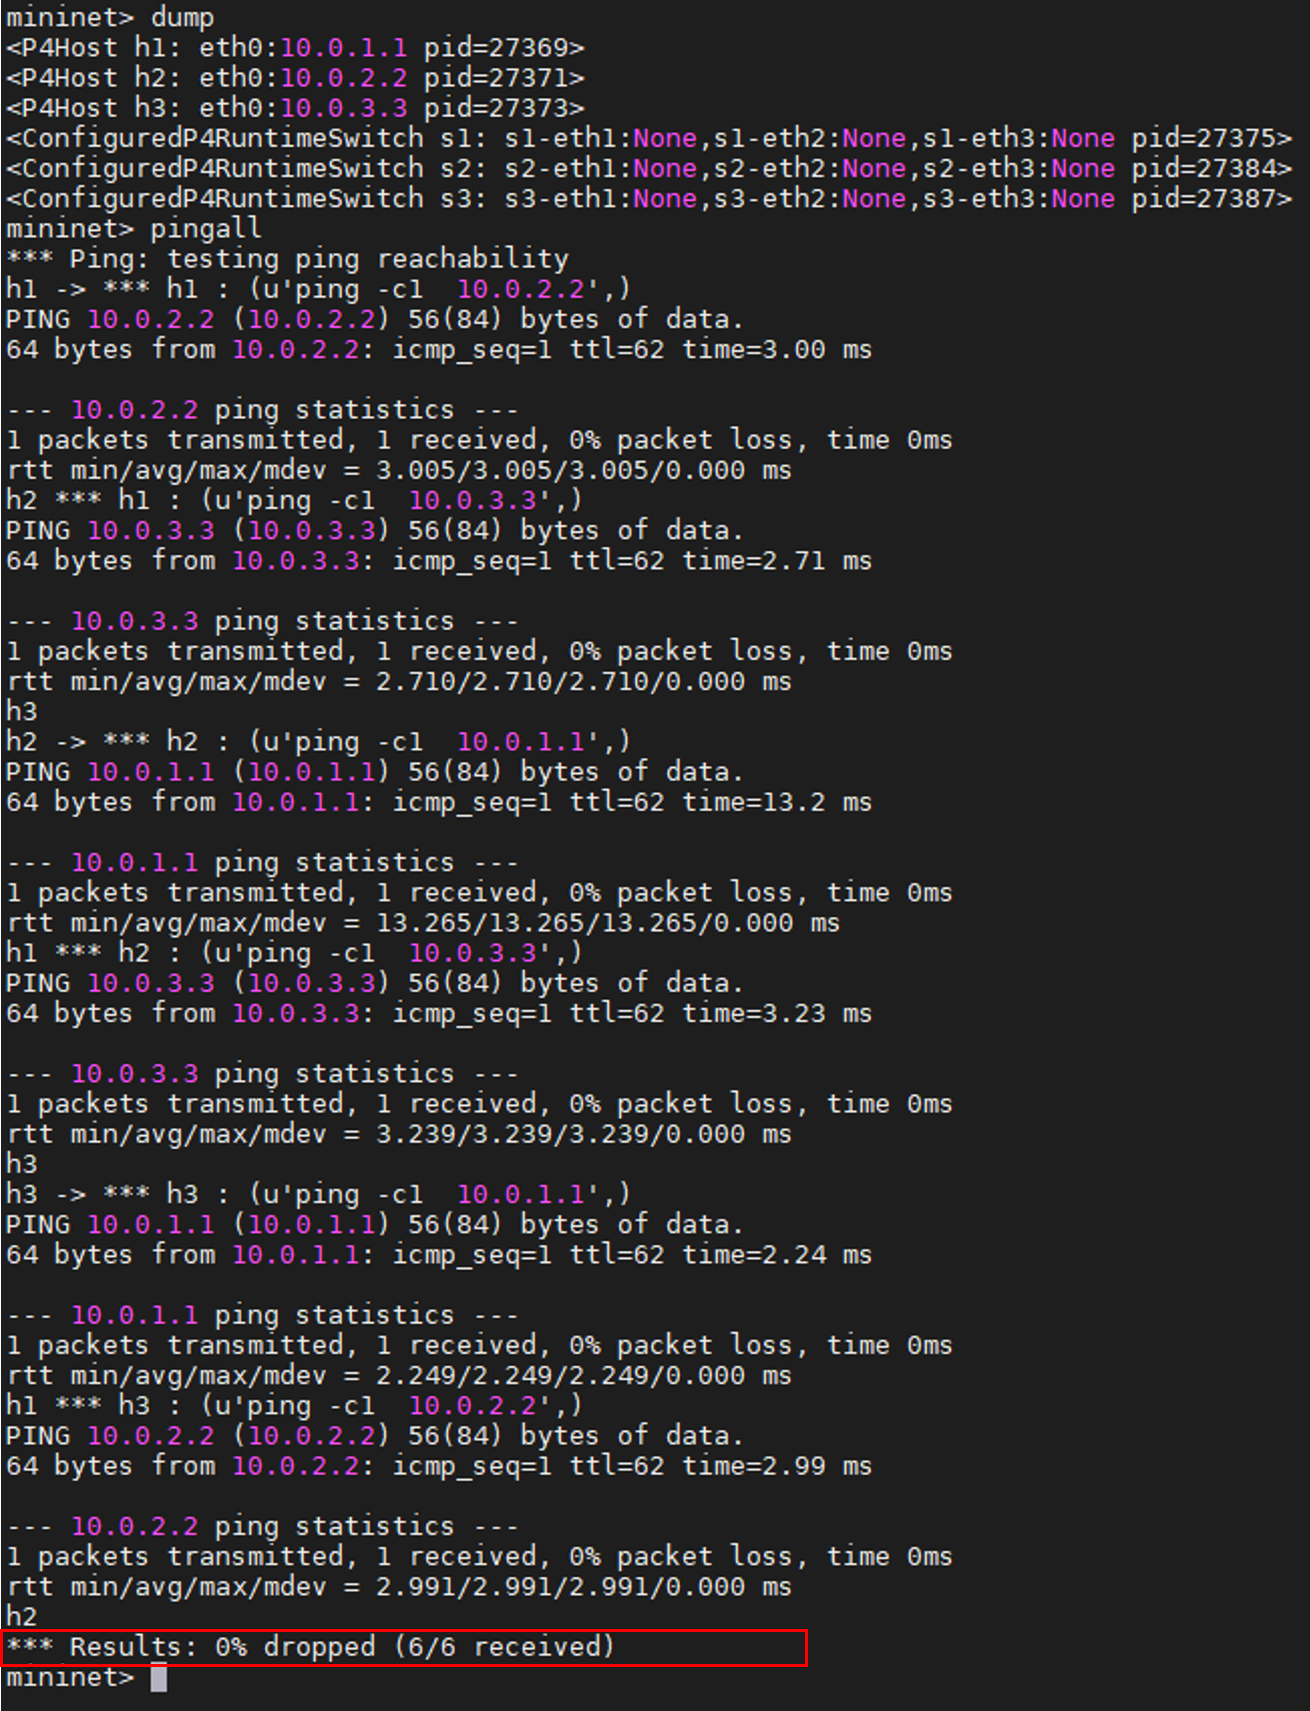
\includegraphics[width=12cm]{archivos/img/dev/p4/case04/demo_case04_edited.png}
    \caption{Comprobación de funcionamiento del Case04 - P4}
    \label{fig:case04_p4_ether_func}
\end{figure}

\newpage

